\documentclass[11pt]{article}

\usepackage[margin=1in]{geometry} 
\usepackage{amsmath,amsthm,amssymb, graphicx, multicol, array}
\usepackage{hyperref}
\usepackage{caption}
\usepackage{subcaption}

\newcommand{\N}{\mathbb{N}}
\newcommand{\Z}{\mathbb{Z}}
 
\newenvironment{problem}[2][Problem]{\begin{trivlist}
\item[\hskip \labelsep {\bfseries #1}\hskip \labelsep {\bfseries #2.}]}{\end{trivlist}}

\begin{document}
CSCI181AF: Advanced Data Structures\\
09/21/2022
\begin{center}
    \bf{Hash Flooding Experiment}
\end{center}
\vspace{-4mm}
\subsection*{Introduction}
\vspace{-2mm}
This experiment tests the severity of a "Hash Flooding" attack, a Denial of Service attack that purposefully ties up the CPU of a system exploit the deterministic nature of a hash function by inserting values into a hash table that illicit worst case behavior.
Specifically, we utilized two hash tables implemented as Python dictionaries in two different situations, 1) we insert values that all hash to the same value (using the fact that the Python hash function is $n\bmod (2^{61}-1)$ and 2) inserting values that all hash to different values.
\vspace{-4mm}
\subsection*{Data}
\vspace{-2mm}
For our data, we used values of $n = 10,
11,
15,
30,
50,
75,
100,
150,
200,
300,
400,
500,
1000,
1500,
2000,\\
2500,
5000,
7500,
10000,
15000,
20000,
25000,
50000,
75000,
100000,
150000$, from which, we were able to plot each of the corresponding times and generate a plot connecting each of these data points for our control and hash flooding experiments. These numbers were chosen 
to effective compare the runtimes for small values of $n$, and then to visualize the divergence of the two experiments (hence why there is a cluster of smaller values), and then to see how the HashFlooding runtime increased for $n \geq 5000$.
\begin{figure}[h!]
    \begin{center}
        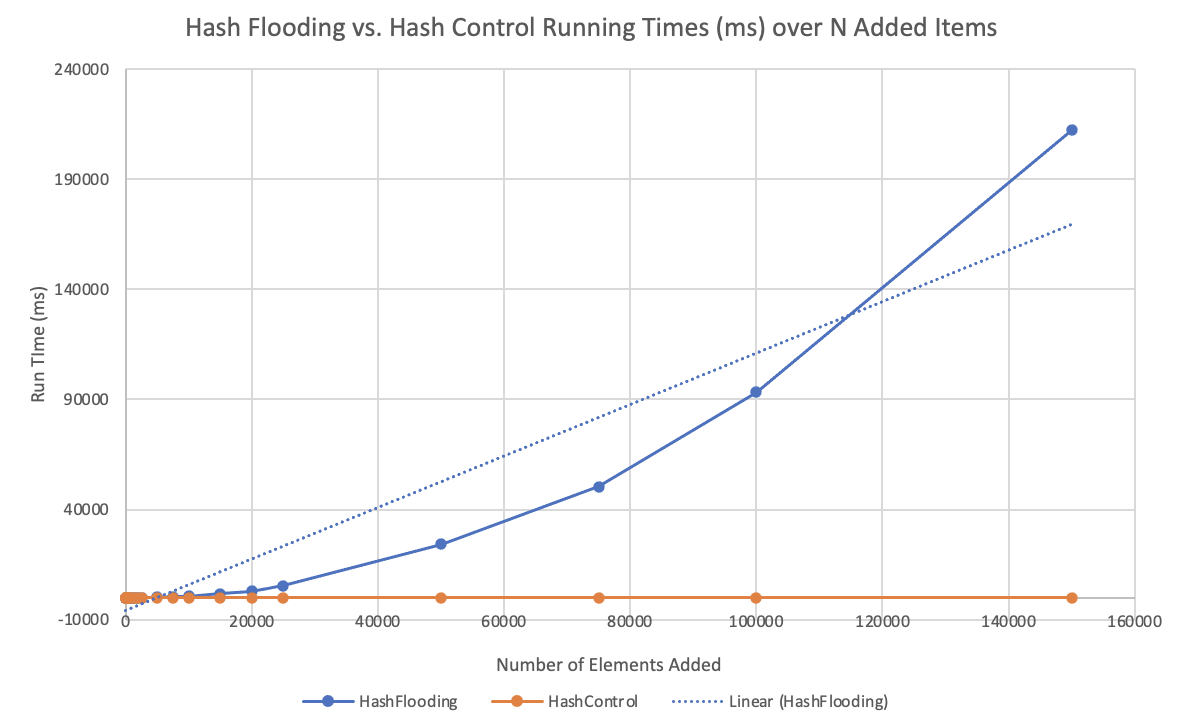
\includegraphics[scale = 0.6]{hashFloodingGraph.png}
    \end{center}
    \caption{Running Time (ms) of Inserting $n$ Items into Hash Tables}
\end{figure}
\vspace{-5mm}
\subsection*{Analysis}
\vspace{-2mm}
Looking at our data, we can see a clear illustration of the effect of Hash Flooding. We can see that inserting $n$ different elements, there seems to be minimal changes to the runtime beyond a 
linear increase that is dwarfed by our flooding case. It is noticeable that while the Hash Flooding experiment begins around the same runtime as that of our control experiment, there is a rapid increase 
as $n$ increases that appears to be a non-linear run-time. Therefore, we can see that by choosing a large number (say 150,000) values that hash to the same hash value,
one can very effectively occupy the CPU of a computer for a large amount of time.
\end{document}